\documentclass[12pt]{article}
\usepackage[margin=1in]{geometry}
\usepackage{times}
\usepackage{natbib}
\usepackage{setspace}
\usepackage{url}
\setcitestyle{authoryear,open={(},close={)}}
\onehalfspacing
\usepackage{graphicx} 
\usepackage{amsmath}
\usepackage{amssymb}
\usepackage{forest}
\usepackage{float}
\usepackage{caption}

\begin{document}

\title{An In-Depth Analysis of the Markowitz Portfolio Model}
\author{}
\date{}
\maketitle

\section{Introduction}
The Markowitz Portfolio Model, also known as Modern Portfolio Theory (MPT), revolutionized the field of finance by introducing a quantitative framework for portfolio construction (Markowitz, 1952). This model provides investors with a systematic approach to selecting a combination of assets that optimizes the trade-off between risk and return. By incorporating diversification and assessing asset correlations, investors can potentially lower overall portfolio risk while achieving desirable returns (Encyclopaedia Britannica, n.d.; Markowitz, 1952). 

The theoretical underpinnings of the model shifted investment analysis from a predominantly qualitative exercise to one that is grounded in rigorous mathematics. Prior to its inception, portfolio selection was based largely on historical performance and subjective judgment. Markowitz's pioneering work introduced the concept that risk, measured by the variance of returns, could be quantitatively analyzed and managed. This marked a significant departure from traditional approaches and has since paved the way for the development of advanced investment strategies and financial products (Markowitz, 1952).

Furthermore, the model has not only enhanced the academic discourse surrounding asset allocation but has also transformed practical investment management. Its emphasis on diversification and optimization has influenced a broad range of applications, from mutual fund management to the construction of hedge funds portfolios. In academic research, the Markowitz model has been instrumental in inspiring subsequent studies on risk management and efficient market hypotheses (Encyclopaedia Britannica, n.d.). Its robust framework continues to serve as a cornerstone for both theoretical exploration and empirical testing in finance. The comprehensive nature of the model allows for its adaptation across different market conditions, demonstrating its enduring relevance in a rapidly evolving financial landscape.

The introduction of Modern Portfolio Theory has had far-reaching implications, not only in how investments are managed but also in how risk is perceived and quantified. The adoption of statistical measures such as expected return and standard deviation has set a new standard for evaluating investment performance, thereby enabling a more scientific approach to financial decision-making (Markowitz, 1952). This paradigm shift has encouraged continuous refinement and expansion of portfolio theories, fostering innovation and development in the field of quantitative finance.

\section{Background}
Harry Markowitz's seminal work, published in 1952 in the \textit{Journal of Finance}, laid the foundational principles for Modern Portfolio Theory by formalizing the concept of diversification as an effective risk management tool (Markowitz, 1952). His article, ``Portfolio Selection,'' demonstrated that investors could reduce unsystematic risk by carefully selecting a mix of assets that do not exhibit perfect positive correlations. This innovative approach not only redefined portfolio management but also introduced a rigorous analytical framework that continues to influence both academic research and practical investment strategies (Markowitz, 1952).

Markowitz’s groundbreaking ideas emerged during a period when the financial markets were beginning to embrace quantitative methods. At the time, the prevailing investment strategies were largely based on anecdotal evidence and historical performance, which often led to suboptimal decision-making. By applying statistical techniques to assess the relationship between risk and return, Markowitz provided investors with a more reliable and systematic method for constructing portfolios. This paradigm shift has been widely acknowledged as a turning point in the history of financial economics (Encyclopaedia Britannica, n.d.).

The impact of his work was further cemented by the recognition it received from the academic community and industry practitioners alike. In 1990, Harry Markowitz was awarded the Nobel Prize in Economic Sciences for his contributions, an honor that underscored the significance of his research in advancing financial theory (Nobel Prize, 1990). His model not only provided a clear framework for understanding the benefits of diversification but also laid the groundwork for subsequent developments in portfolio optimization and asset pricing. Over the decades, the model has been refined and extended by numerous scholars, solidifying its role as a fundamental concept in modern investment analysis (Encyclopaedia Britannica, n.d.).

Moreover, the principles set forth by Markowitz have found extensive applications beyond traditional portfolio management. They have influenced the design of risk management systems, the evaluation of financial instruments, and the formulation of regulatory policies in global financial markets. The methodological rigor introduced by his work continues to inspire innovations in the field, ensuring that the model remains at the forefront of financial theory and practice (Markowitz, 1952). The enduring legacy of the Markowitz Portfolio Model is evident in its widespread adoption and its continual relevance in both academic literature and real-world investment strategies.

\newpage

\section{Purpose and Key Concepts}
The primary purpose of the Markowitz Portfolio Model is to assist investors in constructing portfolios that maximize expected returns for a given level of risk, or conversely, minimize risk for a predetermined return (Markowitz, 1952). At the heart of this approach is the principle of diversification, which posits that investing in a variety of assets with low or negative correlations can significantly reduce overall portfolio volatility (Encyclopaedia Britannica, n.d.; Markowitz, 1952).

\subsection*{Key Concepts}
\paragraph{Risk and Return.} The model evaluates investments based on their expected returns and the standard deviation of these returns. The expected return provides an estimate of the average outcome, while the standard deviation quantifies risk through the volatility of returns (Markowitz, 1952). This dual consideration is crucial for assessing the attractiveness of different investment opportunities.

\paragraph{Efficient Frontier.} The concept of the efficient frontier represents the set of optimal portfolios that offer the highest expected return for a given level of risk, or the lowest risk for a specified level of return. Portfolios lying on the efficient frontier are deemed efficient because any deviation from this set results in a suboptimal risk-return trade-off (Encyclopaedia Britannica, n.d.).

\paragraph{Diversification.} Diversification involves spreading investments across a range of asset classes to mitigate unsystematic risk. By combining assets that do not move perfectly in tandem, the negative impact of a single asset’s poor performance is reduced, leading to a more stable overall portfolio (Markowitz, 1952; Encyclopaedia Britannica, n.d.).

\paragraph{Risk Aversion.} The model is predicated on the assumption that investors are risk-averse, meaning that for any given level of expected return, investors prefer the portfolio with lower risk. This assumption underlies the rationale for diversification and the pursuit of the efficient frontier, as it compels investors to seek a balance that minimizes potential losses while targeting acceptable returns (Markowitz, 1952).

\section{Methodology}
This project implements the Markowitz Mean-Variance Optimization framework to construct an optimal portfolio using historical stock data from 10 major publicly traded companies. The primary objective is to identify portfolios with minimum risk under different constraints.

\subsection*{Data Collection and Preprocessing}
Daily adjusted closing prices were retrieved from Yahoo Finance for the period from January 1, 2024 to January 1, 2025 for the following companies: TSLA, AMZN, META, JNJ, XOM, JPM, KO, INTC, NFLX, and PG. The adjusted prices account for stock splits and dividends, providing a consistent basis for return calculations. \\
The daily logarithmic returns were calculated for each stock using the formula:
\[R_t=\log \left (\frac{P_t}{P_{t-1}} \right )\]
These log returns were then cleaned to remove any missing values. Descriptive statistics, such as the mean return (expected return), standard deviation (volatility), correlation, and covariance matrices, were computed and used as inputs to the portfolio optimization problem.

\subsection*{Portfolio Optimization}
Two portfolio optimization models were implemented:

\subsubsection*{1. Minimum Variance Portfolio}
This model minimizes the portfolio variance:
\[\text{minimize } \mathbf{w^T\Sigma w}\]
subject to the constraint:
\[\sum_{i=1}^n w_i=1\]
where $\mathbf{w}$ is the vector of portfolio weights, and $\mathbf{\Sigma}$ is the sample covariance matrix of returns. Short-selling is allowed in this model, so weights can be negative.

\subsubsection*{2. Minimum Variance Portfolio without shortselling}
This model introduces a non-negativity constraint to the previous optimization problem:
\[w_i \geq 0 \quad \text{for all i}\]
This formulation prevents short-selling, meaning the investor can only hold long positions in assets.\newline
Both optimization problems were solved using the solve.QP() function from the quadprog package in R.

\section{Results and Discussion}
Two optimal portfolios were computed using the Markowitz mean-variance framework: one allowing short-selling and one prohibiting it. Their expected return and risk characteristics are summarized below.
\subsection*{1. Minimum Variance Portfolio (with Short-Selling)}
The optimal portfolio under this model includes both long and short positions. The expected performance metrics are:
\begin{itemize}
    \item \textbf{Expected Daily Log Return:} $\sim 0.000678$
    \item \textbf{Expected Normalized Annual Return:} $\sim 18.64\%$
    \item \textbf{Portfolio Standard Deviation (Risk):} $\sim 0.005342$
\end{itemize}
\begin{figure} [h]
    \centering
    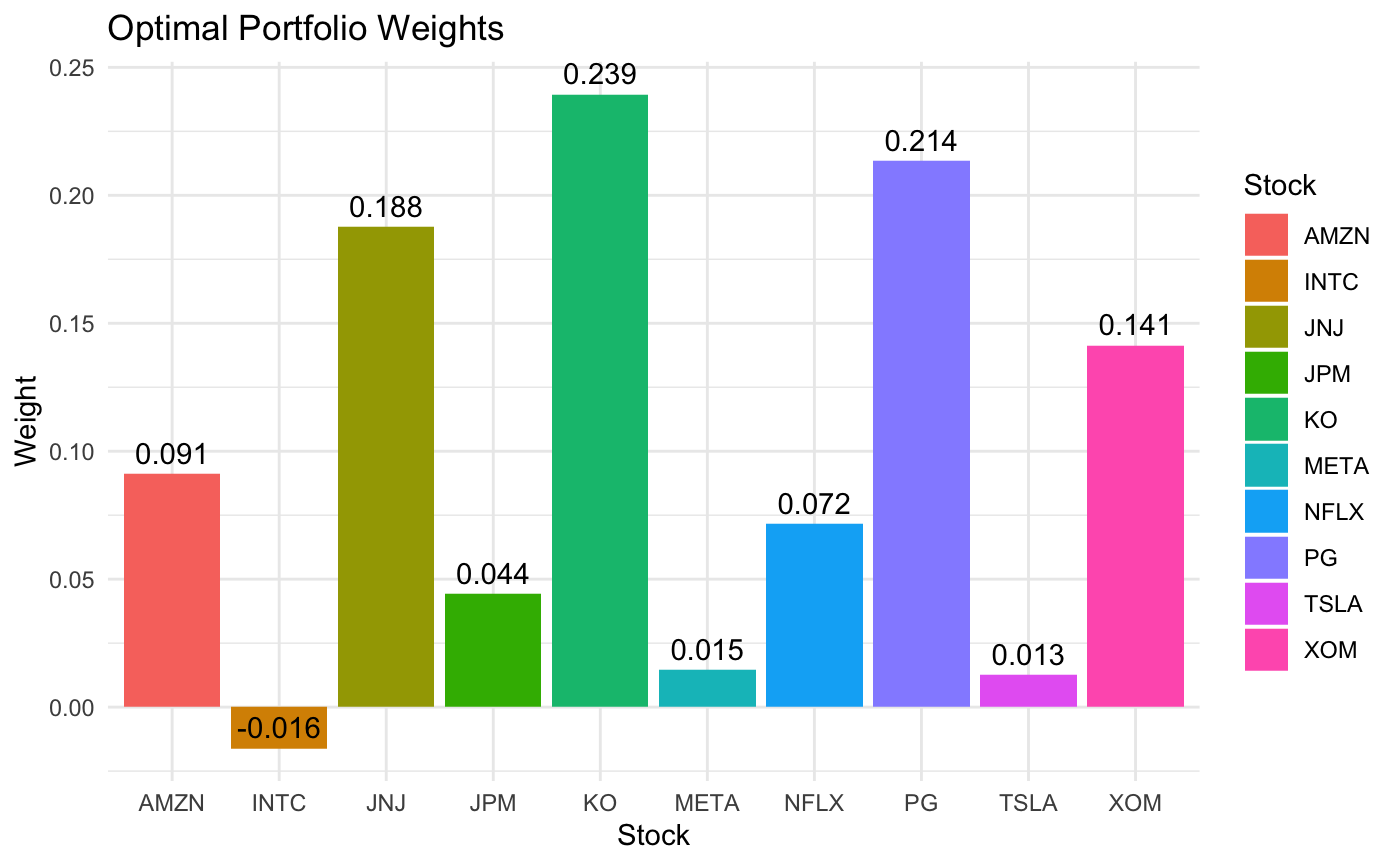
\includegraphics[width=0.6\linewidth]{Findings_Yutong/weights.png}
    \caption{Optimal Weights}
    \label{opt weights}
\end{figure}

\subsection*{2.  Minimum Variance Portfolio (No Short-Selling)}
Under the restriction that all portfolio weights must be non-negative, the optimized portfolio yields:
\begin{itemize}
    \item \textbf{Expected Daily Log Return:} $\sim 0.000594 $
    \item \textbf{Expected Normalized Annual Return:} $\sim 16.16\%$
    \item \textbf{Portfolio Standard Deviation (Risk):} $\sim 0.005362$
\end{itemize}
\begin{figure}[H]
    \centering
    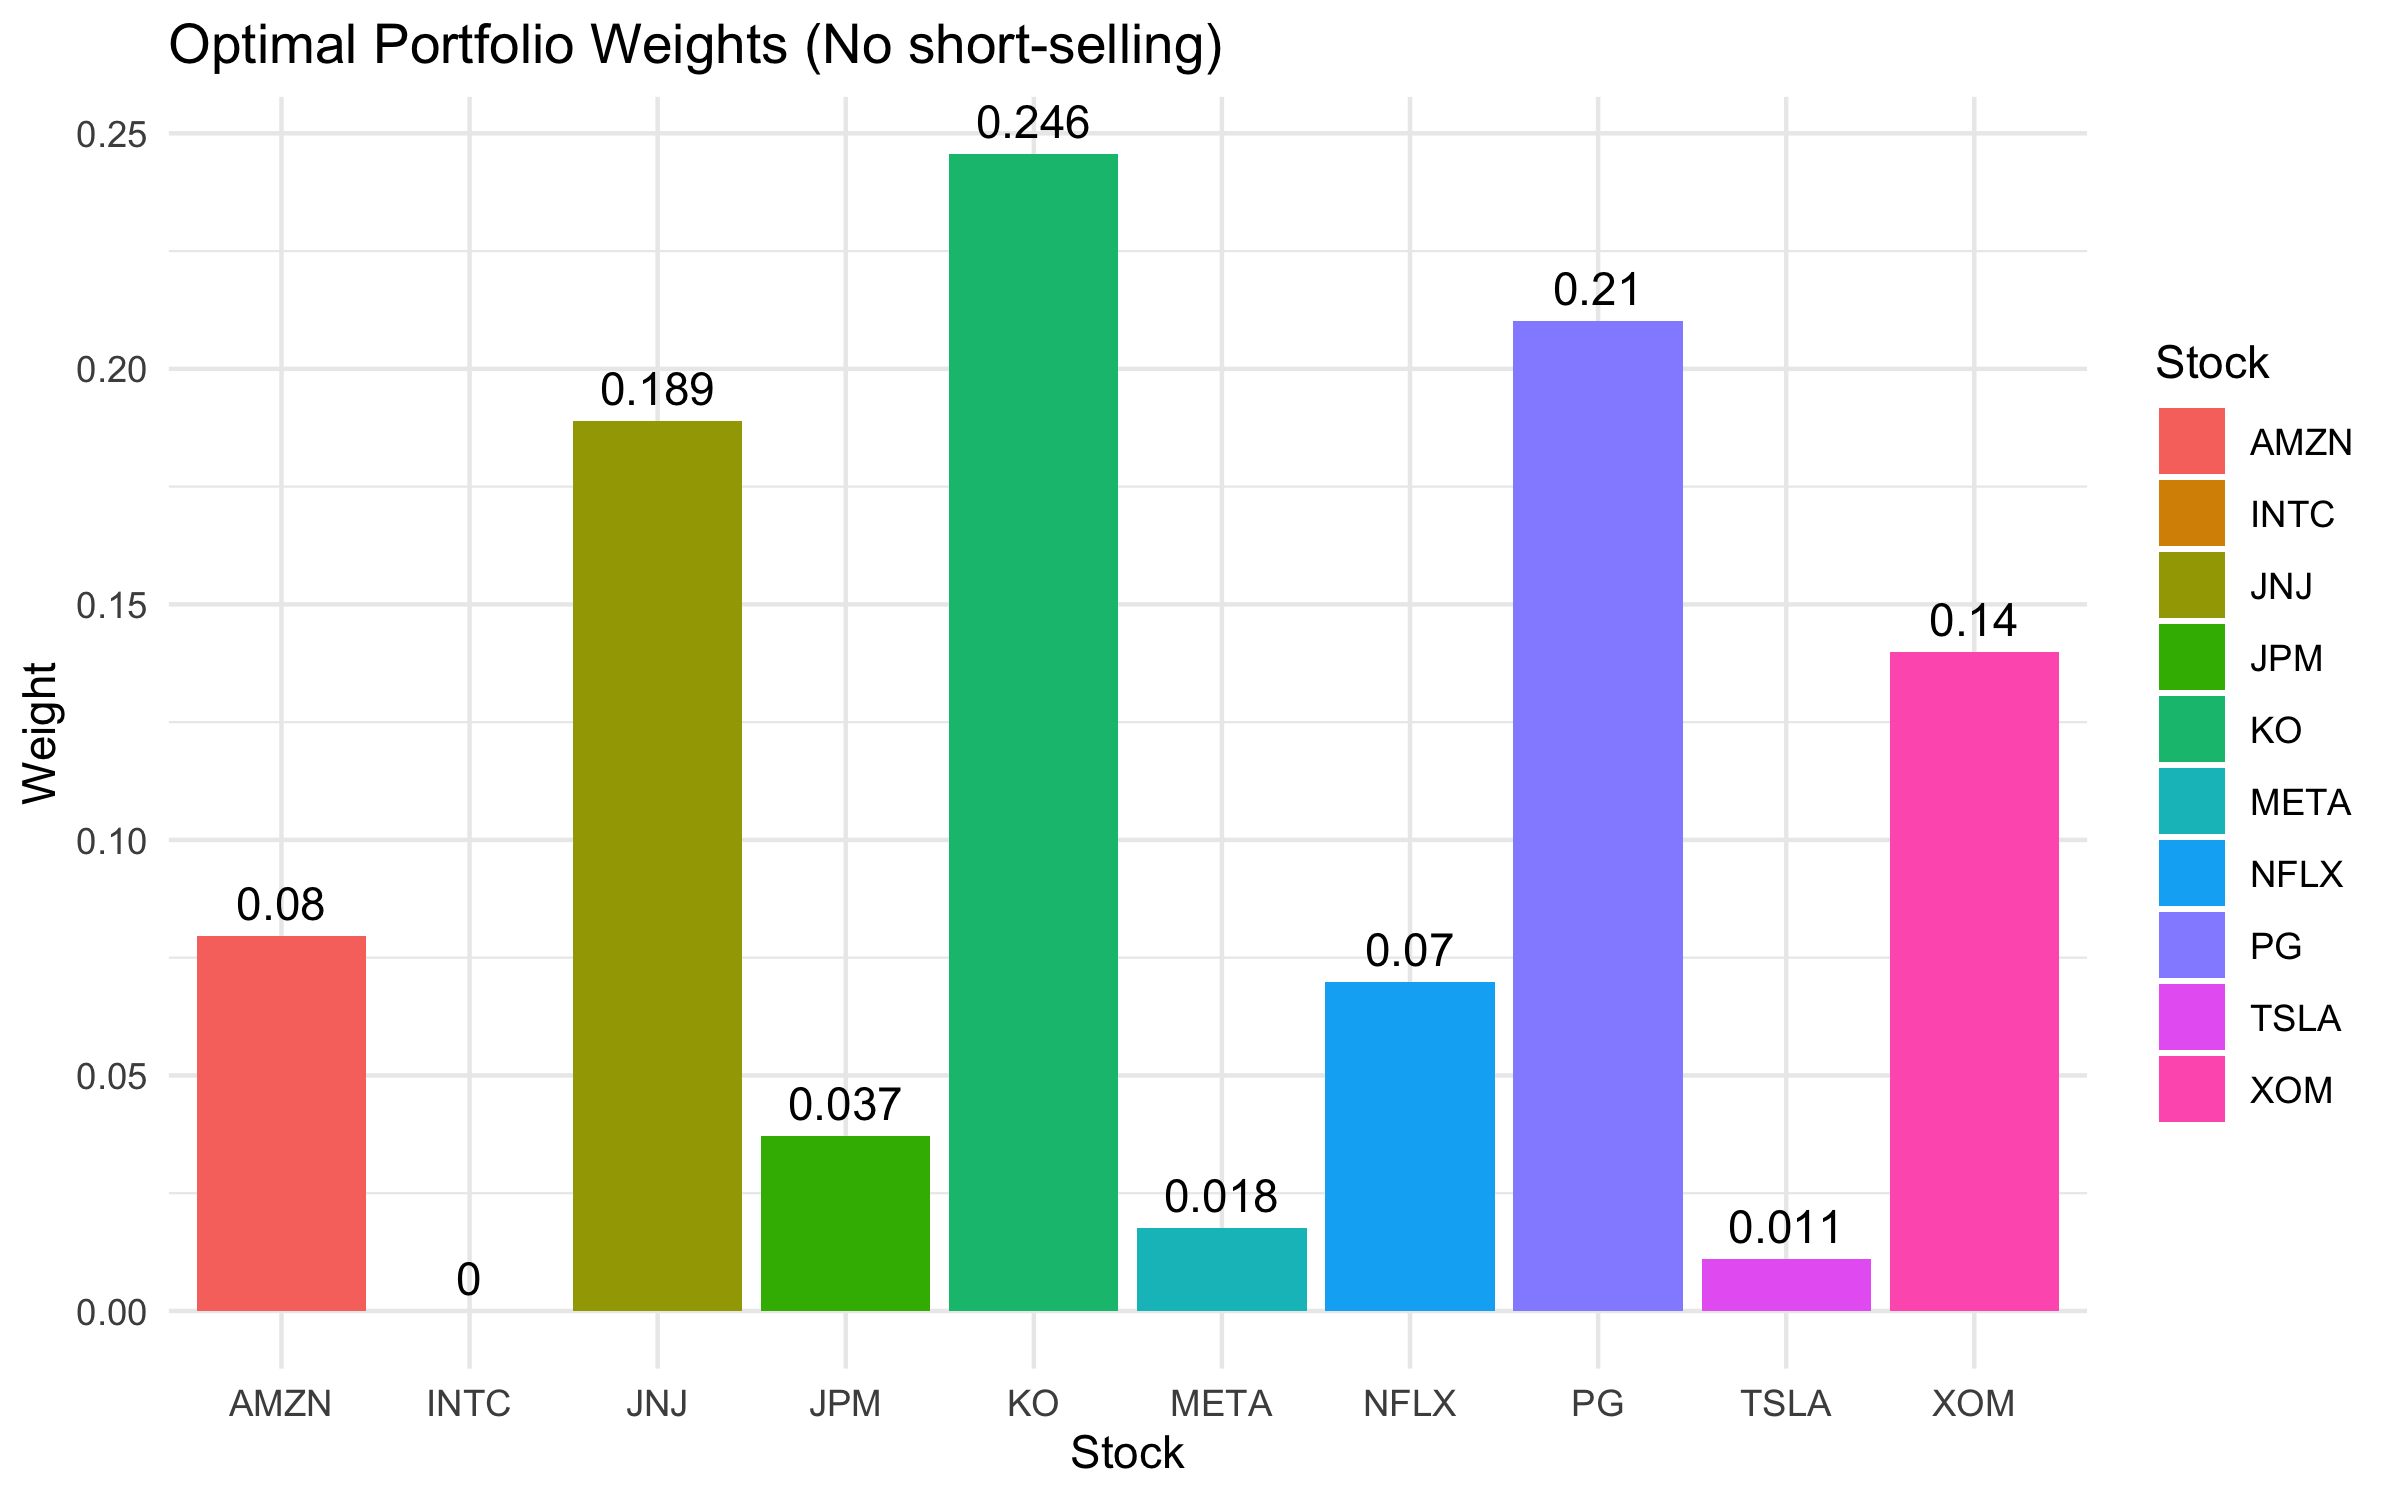
\includegraphics[width=0.6\linewidth]{Findings_Yutong/portfolio_weights_plot.png}
    \caption{Optimal Weights (No Short-Selling)}
    \label{opt weights no}
\end{figure}
As expected, the restriction on short-selling increases the portfolio's variance slightly. The return is also marginally lower than the unconstrained portfolio. However, this version is more applicable to risk-averse or institutional investors who are prohibited from short-selling.

\subsection*{Efficient Frontier}
A Monte Carlo simulation of 10,000 randomly generated portfolios was conducted to visualize the efficient frontier. The efficient frontier graph displays the risk-return trade-off and confirms that the optimized portfolios lie on the lower edge of the cloud—indicating they are mean-variance efficient.
\begin{figure}[H]
    \centering
    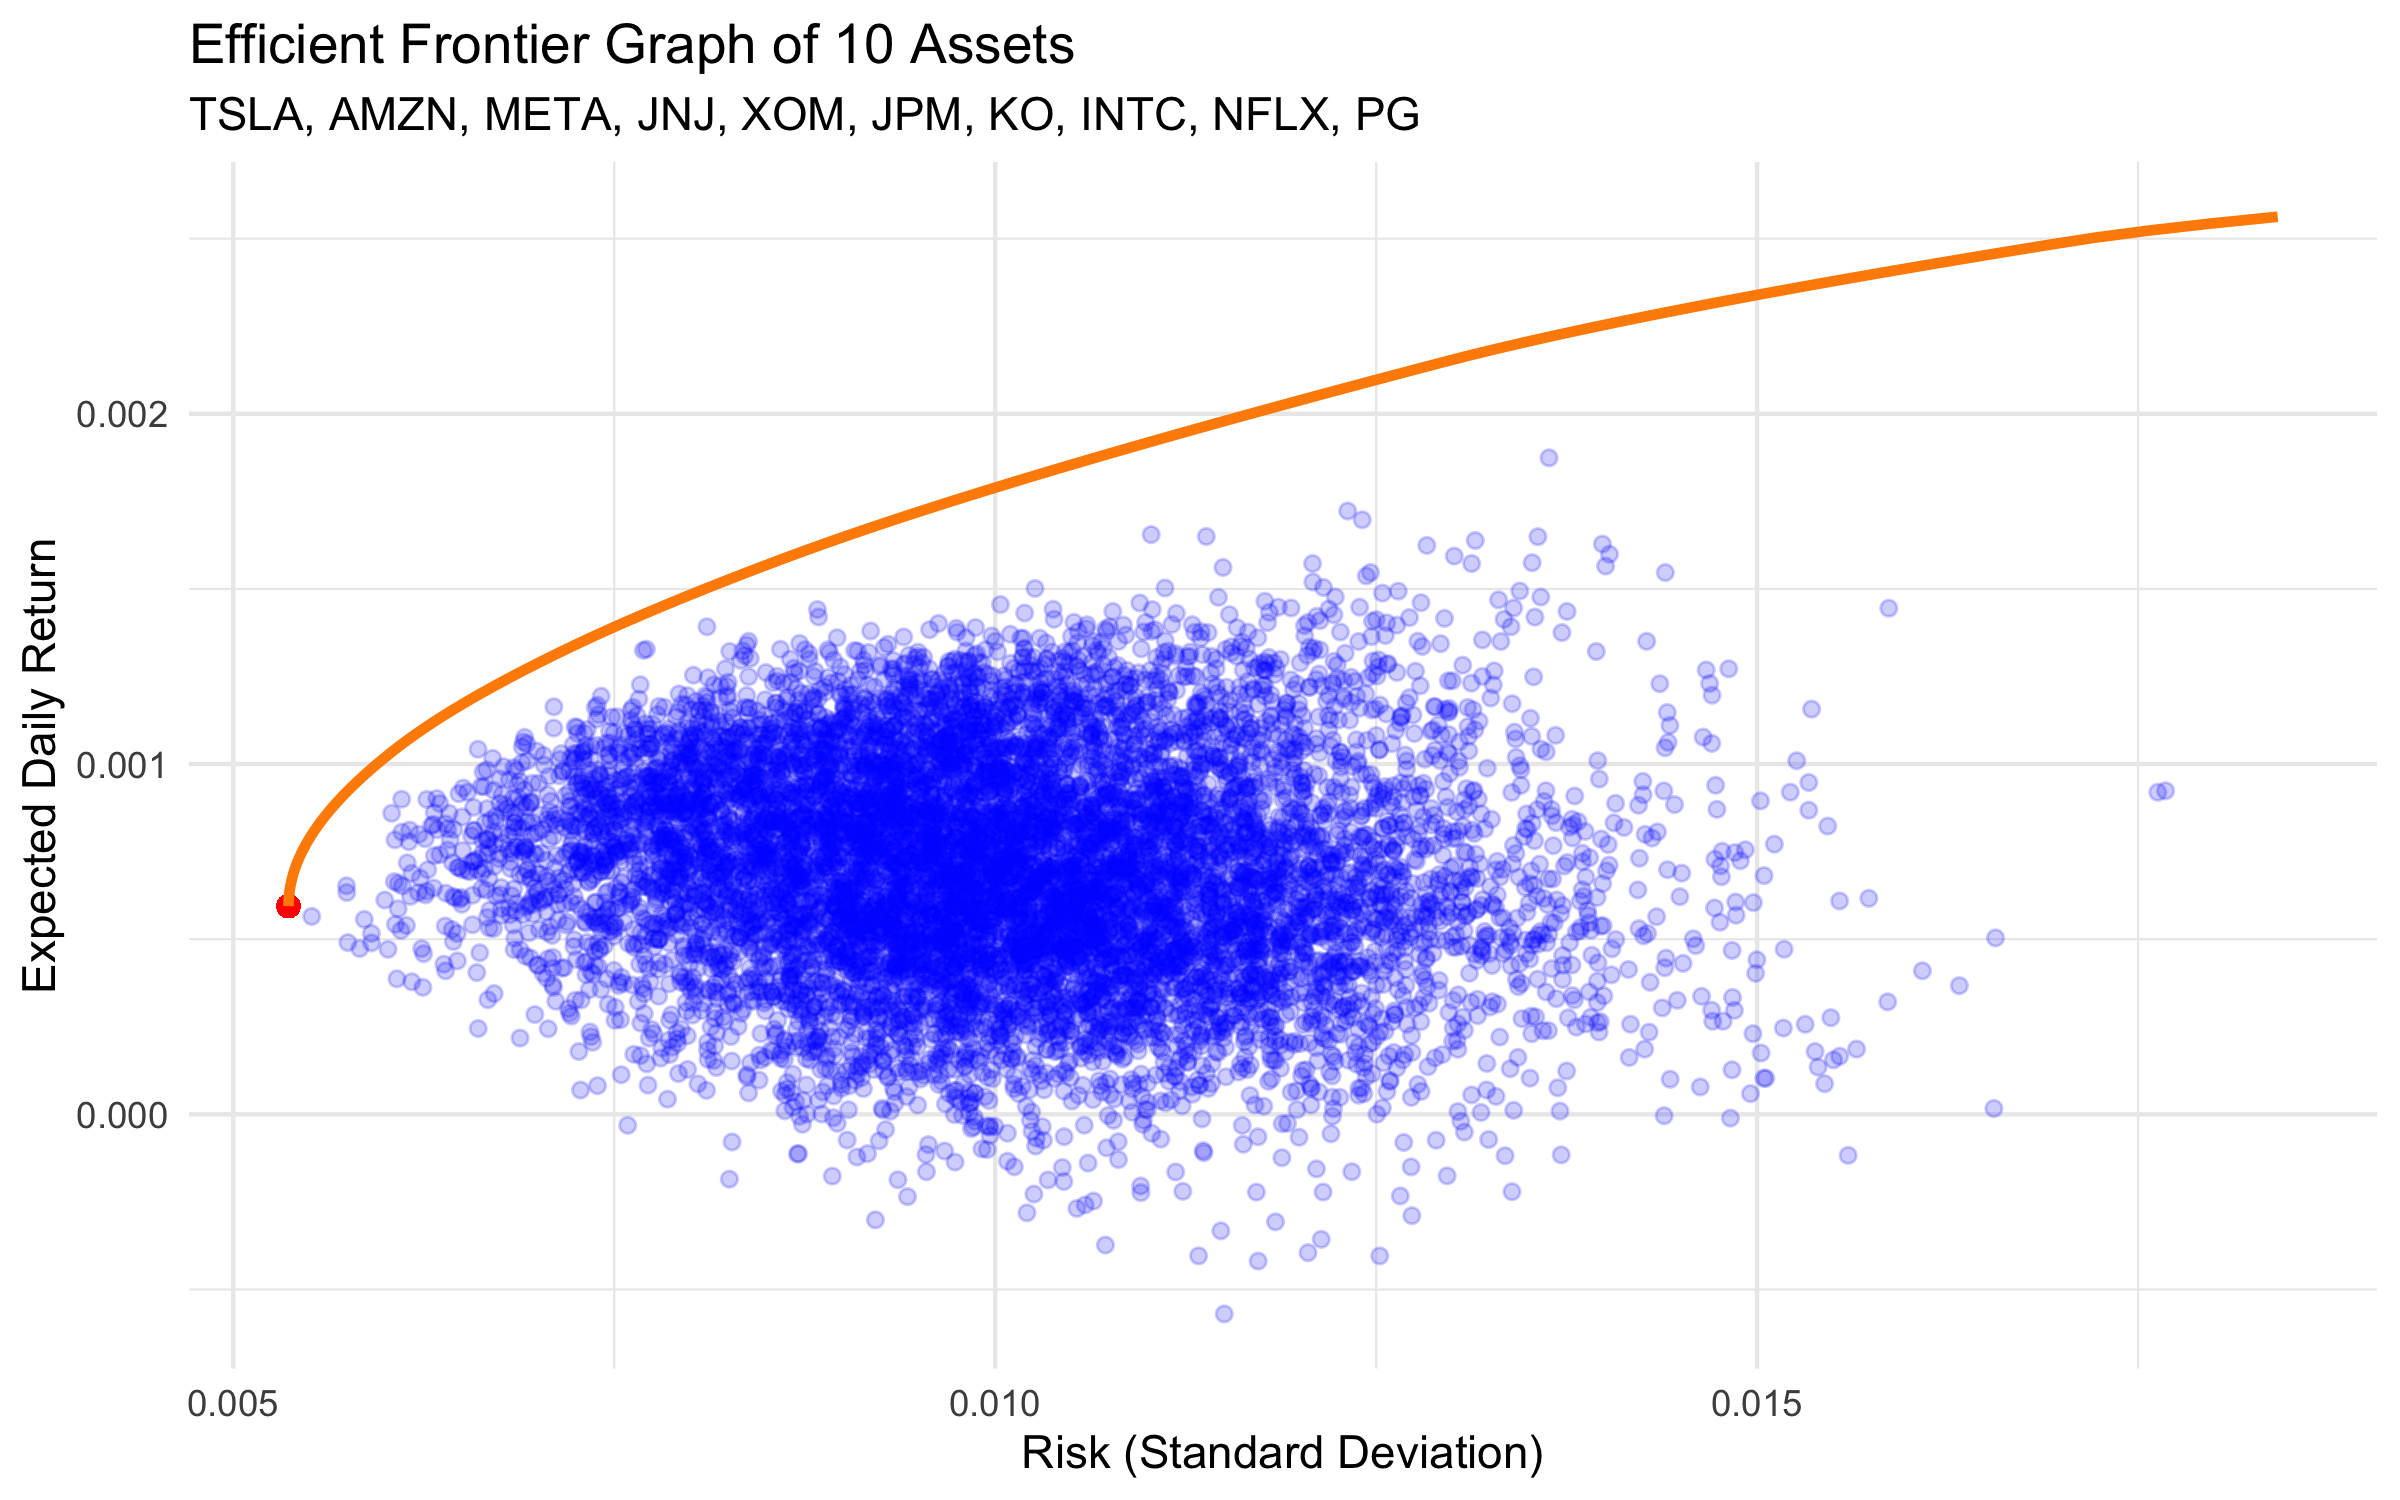
\includegraphics[width=0.6\linewidth]{Findings_Yutong/efficient_frontier_plot.png}
    \caption{Efficient Frontier}
    \label{eff-fro}
\end{figure}
The orange curve represents the efficient frontier, which consists of all portfolios that provide the highest possible return for a given level of risk, or equivalently, the lowest possible risk for a given level of return. Portfolios on this frontier are considered mean-variance efficient and are preferred over those below it.\par
The red dot on the far left of the orange curve represents the global minimum variance (GMV) portfolio, which has the lowest possible risk among all feasible portfolios. This portfolio is often used as a reference point in portfolio theory because it minimizes volatility without regard to return.\\
\textbf{Key Observations:}
\begin{itemize}
    \item All of the simulated portfolios lie below the efficient frontier, indicating suboptimal combinations of risk and return.
    \item The efficient frontier is upward-sloping and concave, reflecting the trade-off between risk and return: higher expected returns can be achieved, but only at the cost of increased risk.
    \item Portfolios above the frontier are infeasible under current assumptions and constraints.
    \item The diversification effect is clearly visible: random combinations tend to reduce overall risk due to the covariance between assets, clustering most portfolios in a dense middle region.
\end{itemize}

\subsection*{Cumulative Return Comparison}
The cumulative return curves represent the normalized portfolio growth over time, computed by exponentiating the cumulative sum of actual daily log returns. This effectively models how a \$1 investment would evolve over the course of the year, accounting for compound growth.
\begin{figure} [H]
    \centering
    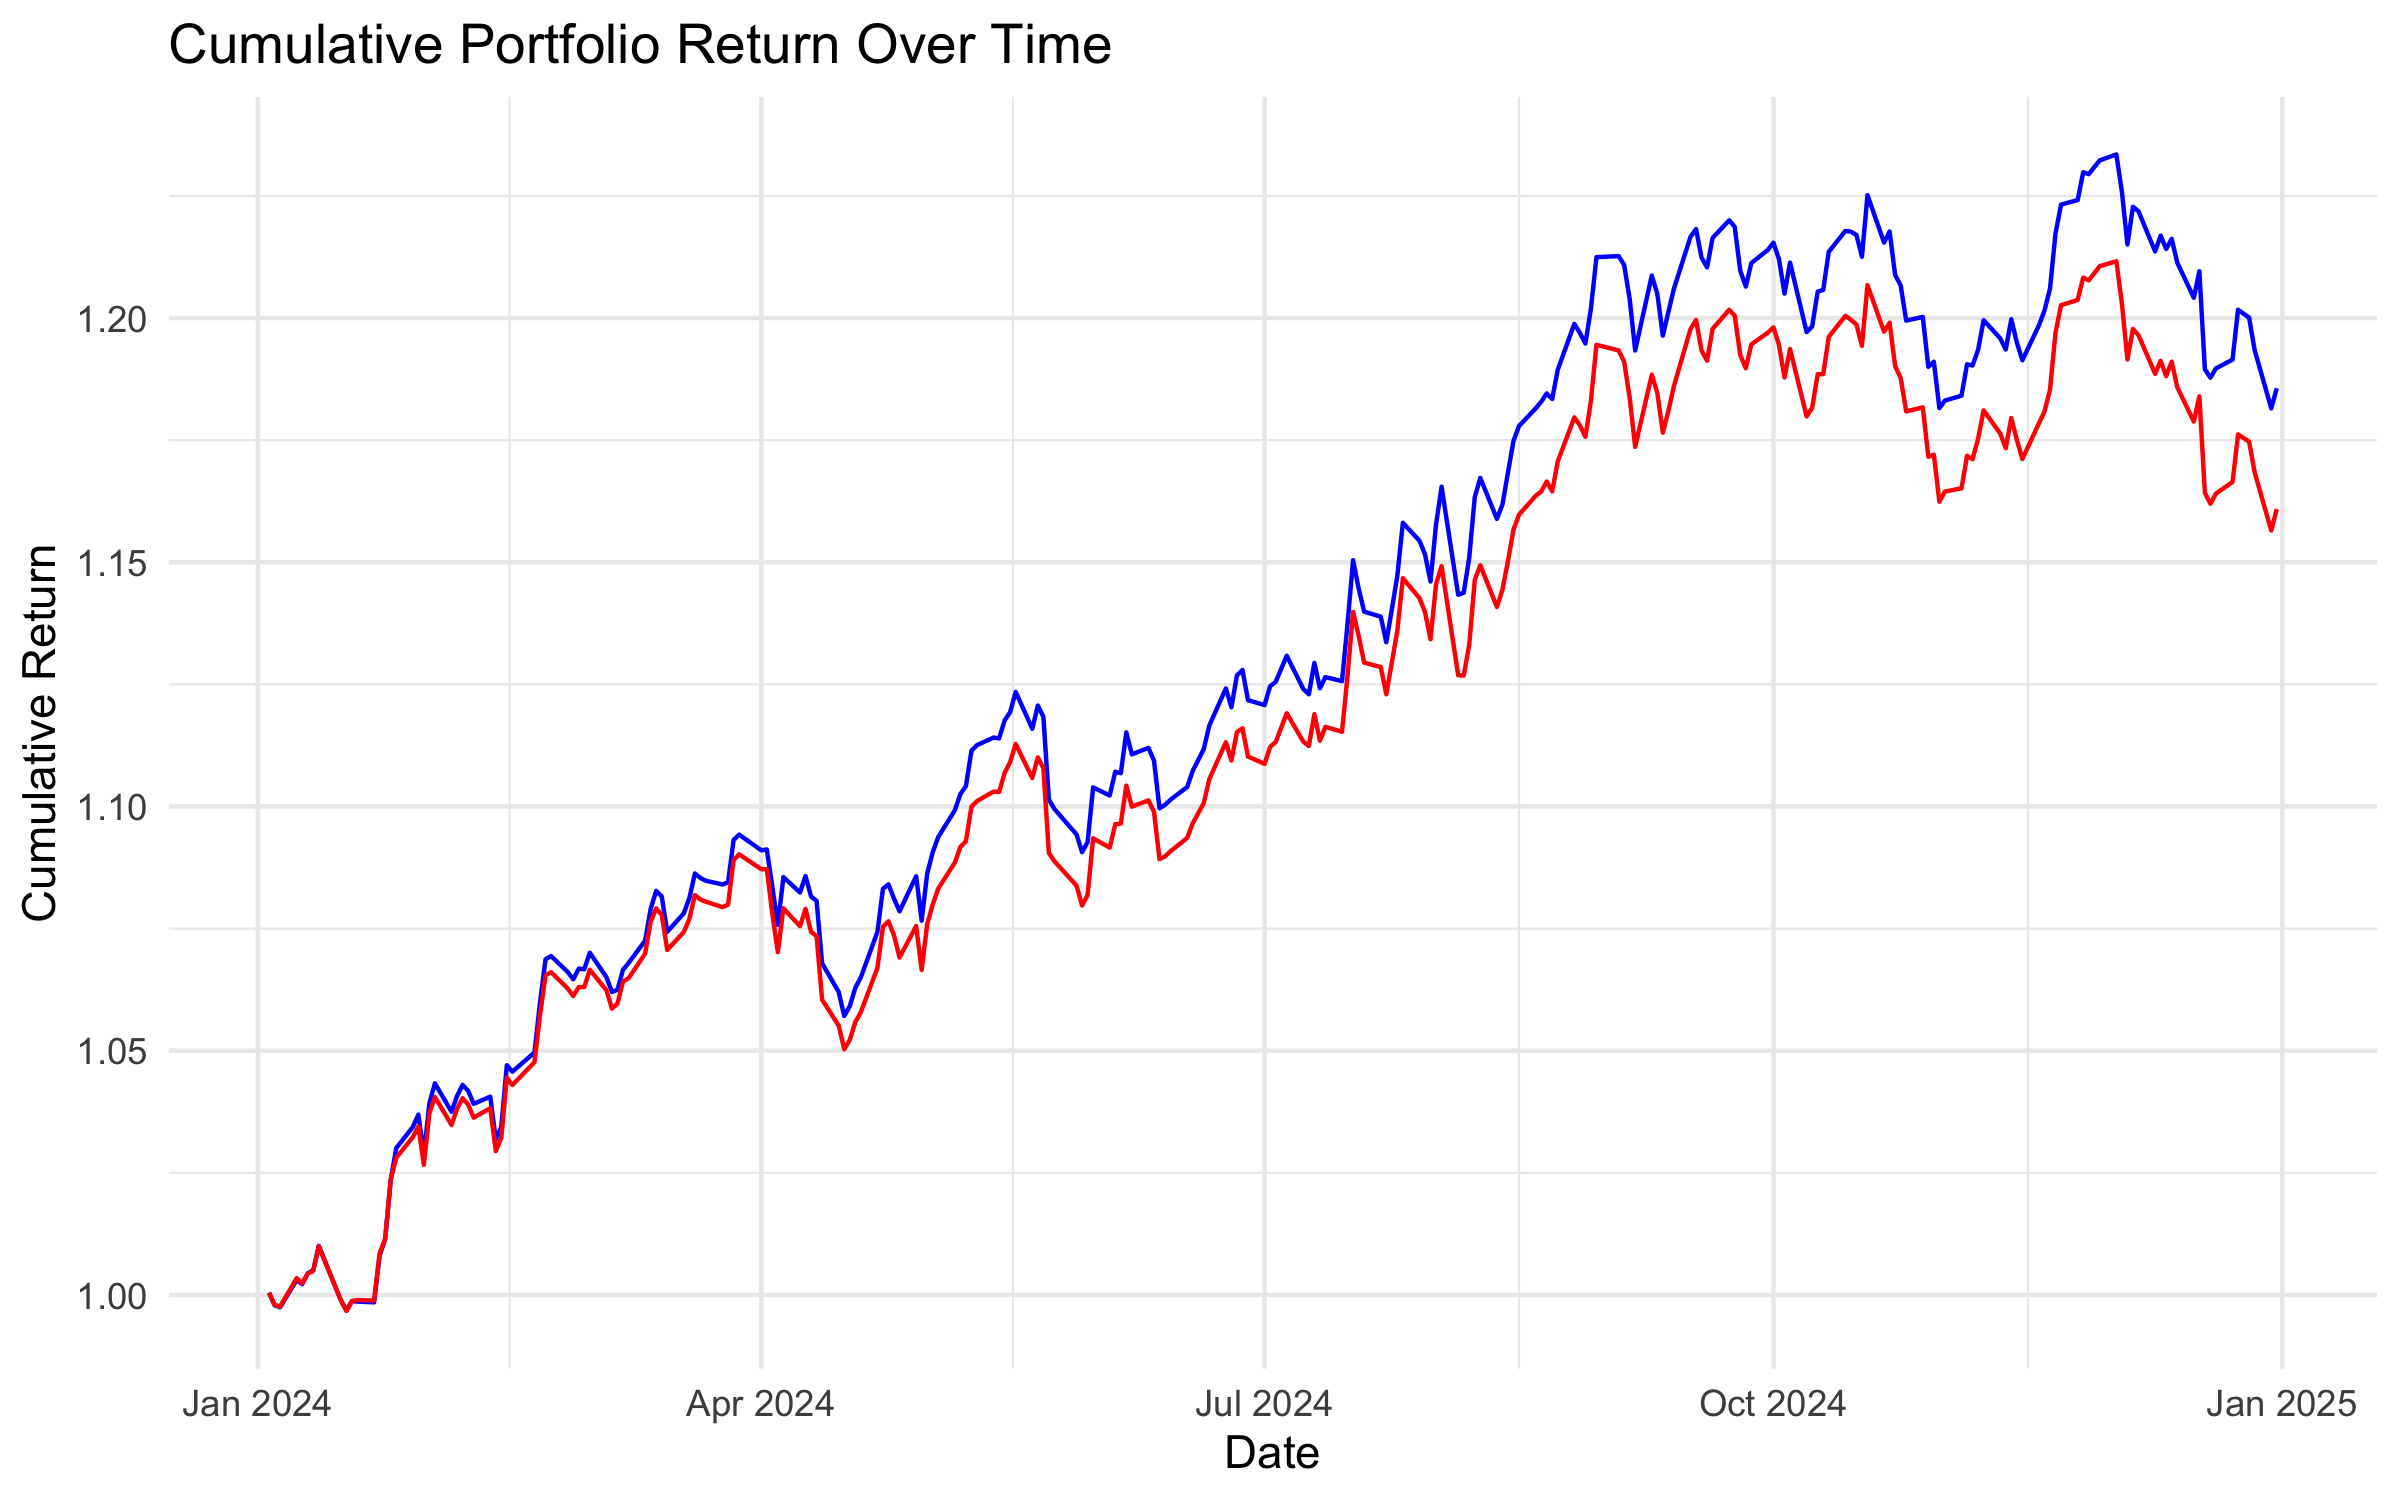
\includegraphics[width=0.6\linewidth]{Findings_Yutong/cumulative_return.png}
    \caption{Cumulative Return}
    \label{cum-return}
\end{figure}
The figure above shows the cumulative returns of the two optimized portfolios over the course of 2024:
\begin{itemize}
    \item \textbf{Blue Line:} Minimum Variance Portfolio with short-selling allowed.
    \item \textbf{Red Line:} Minimum Variance Portfolio without short-selling (long-only).
\end{itemize}
     \paragraph{General Trend:} Both portfolios exhibit a positive growth trend, indicating that the optimized portfolios yielded positive returns over the year. This aligns with the earlier result where both had positive expected annual returns.
    \paragraph{Commonalities:}The two portfolios move in broadly the same direction, reacting similarly to market trends. Both lines show periods of faster and slower growth, reflecting the influence of market-wide factors affecting all assets.
    \paragraph{Differences:} The blue line (with short-selling) generally lies slightly above the red line throughout the year, showing that allowing short-selling resulted in slightly higher cumulative returns. The performance gap widens at certain periods, suggesting that the flexibility to short-sell enabled the portfolio to better adapt to market conditions—especially during downtrends or volatile periods.

\paragraph{Comparison with Expected Annual Returns:}
Earlier in the analysis, the expected normalized annual returns were calculated from daily log returns using:
\[R_{annual}=\exp(252\times \bar{r}_{daily})-1\]
\begin{itemize}
    \item For the with-short-selling portfolio, the expected annual return was $\sim 18.64\%$
    \item For the no-short-selling portfolio, the expected return was $\sim 16.16\%$
\end{itemize}
These values represent theoretical expectations under assumptions of return stationarity and log-normal behavior.\par
However, the cumulative return plot reflects realized performance over the year. While closely aligned with the expected returns, the cumulative curves account for actual day-to-day compounding and market behavior—thus offering a more intuitive and visual understanding of how the portfolios performed in practice.

\newpage

\begin{spacing}{1.5}
\begin{thebibliography}{9}

\bibitem{britannica_harry_markowitz}
Encyclopaedia Britannica. (n.d.). Harry Markowitz. In \textit{Britannica Money}. Retrieved March 25, 2025, from \url{https://www.britannica.com/money/Harry-Markowitz}

\bibitem{britannica_modern_portfolio_theory}
Encyclopaedia Britannica. (n.d.). Modern portfolio theory. In \textit{Britannica Money}. Retrieved March 25, 2025, from \url{https://www.britannica.com/money/modern-portfolio-theory-explained}

\bibitem{markowitz1952portfolio}
Markowitz, H. M. (1952). Portfolio selection. \textit{Journal of Finance, 7}(1), 77--91.

\bibitem{nobel_prize_harry_markowitz}
Nobel Prize. (1990). The Sveriges Riksbank Prize in Economic Sciences in Memory of Alfred Nobel 1990. In \textit{NobelPrize.org}. Retrieved March 25, 2025, from \url{https://www.nobelprize.org/prizes/economic-sciences/1990/markowitz/facts/}

\end{thebibliography}
\end{spacing}

\end{document}
